% Created 2023-06-07 Wed 11:25
\documentclass[9pt, b5paper]{article}
\usepackage{xeCJK}
\usepackage[T1]{fontenc}
\usepackage{bera}
\usepackage[scaled]{beraserif}
\usepackage[scaled]{berasans}
\usepackage[scaled]{beramono}
\usepackage[cache=false]{minted}
\usepackage{xltxtra}
\usepackage{graphicx}
\usepackage{xcolor}
\usepackage{multirow}
\usepackage{multicol}
\usepackage{float}
\usepackage{textcomp}
\usepackage{algorithm}
\usepackage{algorithmic}
\usepackage{latexsym}
\usepackage{natbib}
\usepackage{geometry}
\geometry{left=1.2cm,right=1.2cm,top=1.5cm,bottom=1.2cm}
\usepackage[xetex,colorlinks=true,CJKbookmarks=true,linkcolor=blue,urlcolor=blue,menucolor=blue]{hyperref}
\newminted{common-lisp}{fontsize=\footnotesize} 
\author{deepwaterooo}
\date{\today}
\title{ET 框架学习笔记(四)--框架总结}
\hypersetup{
  pdfkeywords={},
  pdfsubject={},
  pdfcreator={Emacs 28.2 (Org mode 8.2.7c)}}
\begin{document}

\maketitle
\tableofcontents


\section{IMHandler 接口实现的各种类型消息处理器:需要先理解透彻ETTask 和 ETVoid}
\label{sec-1}
\begin{itemize}
\item ET7 框架里,不知道破框架的开发者出于什么原因,都精减到像没穿衣服一样删除得光秃秃的。。。想搜什么都搜不出来。
\item 可以回去参考前一个游戏参考过的ET-EUI 里有一部分ETVoid 的相关使用,可以用作自己理解 ETTask ETVoid 的源码参考。ET-EUI 现笔记本里没有,可以拉一个下来。
\item 现ET7 里一个ETVoid 的使用也搜不出来。。。框架的开发者发疯了。。。感觉它故意精减压缩,是想要故意挫败打垮别人,
\item 可是真正的程序员开发者,是永远不怕困难的开发者。爱表哥,爱生活!!!任何时候,活宝妹就是一定要嫁给亲爱的表哥!!!
\end{itemize}
\subsection{IMHandler: interface 消息处理器接口类。它有2 个实现抽象类:AMHandler,AMRpcHandler}
\label{sec-1-1}
\begin{itemize}
\item 实现这个接口类型主要分为两个抽象类:AMHandler,AMRpcHandler
\item 今天上午暂时只看取了这个接口,和两个抽象方法这里。后面任何的个体实现类,都还没有细看,不太懂。
\end{itemize}
\begin{minted}[fontsize=\scriptsize,linenos=false]{csharp}
public interface IMHandler {
    // 下面,返回类型不对
    void Handle(Session session, object message); // 这里返回类型,仍然应该是ETTask, 或者可能的 ETVoid ?
    // 消息处理器帮助类,在程序域加载的时候,会自动扫描程序域里的ActorMessageHander 标签,会想要拿消息的【发送类型】与消息的【返回类型】,来系统化管理消息处理 
    Type GetMessageType();
    Type GetResponseType();// 这里现在想的话,可能存在的问题是:有些消息不带返回类型,那么就是说,那类消息不需要处理吗?它只是不需要返回消息,还是会被通知到的 
}
\end{minted}
\subsection{IMActorHandler: 【仅作参考】大概参考 ET-EUI 来的,它的目的应该是把最基类的接口,与其它两类的接口相区分开来}
\label{sec-1-2}
\begin{itemize}
\item 大概参考 ET-EUI 来的,它的目的应该是把最基类的接口,与其它两类的接口相区分开来。但是,我想、猜测、理解的话,应该是上面一个接口,如果能够把ETTask 与ETVoid 狠好地统一的话,应该一个接口可能可以足以整个框架使用的。
\item 消息处理器:基本可以理解为,总都是【服务端】的消息处理器。【客户端】更多的是发请求消息,和接收消息。客户端狠少涉及什么消息处理。
\item 下面的接口,哪个例子也没有参照,自己改的。极有可能都是错的
\end{itemize}
\begin{minted}[fontsize=\scriptsize,linenos=false]{csharp}
public interface IMActorHandler {
    // 下面,参考的是ET-EUI 可能是 6.0 版本。ET7 里,可能接口还可以简化,还是Actor 消息机制模块简化了,不一定如下面这样
    void Handle(Entity entity, int fromProcess, object actorMessage);
    // ETTask Handle(Entity entity, object actorMessage, Action<IActorResponse> reply);
    Type GetRequestType();
    Type GetResponseType();
}
\end{minted}
\subsection{AMHandler<Message>: abstract 抽象基类:两个方法的返回类型,成为现在全框架的理解与实现难点}
\label{sec-1-3}
\begin{itemize}
\item AMHandler类,这个类相比AMRpcHandler更加简单一些,因为这个类型的处理,不需要关心回消息
\item 实现了接口IMHandler的Handle异步方法,具体逻辑为:
\begin{itemize}
\item 将传进来的msg首先转换为模板类,在AMHandler类里面为Message,具体应该为实现AMHandler的类的具体数据类。
\item 根据数据类,以及session生成一些报错日志,方便调试
\item 调用Run方法,将session及具体的数据类传进去
\item 实际继承抽象类AMHandler的类型,会实现这个接口,从而走向各自的处理。
\begin{minted}[fontsize=\scriptsize,linenos=false]{csharp}
public abstract class AMHandler<Message>: IMHandler where Message : class {

// 虽然我这么改,可以暂时消掉编译错误。但改得不对,现在消掉了编译错误,等编译通过,运行时错误会一再崩出来的。。。
    protected abstract void Run(Session session, Message message); 
    // protected abstract ETTask Run(Session session, Message message);

    // public async ETVoid Handle(Session session, object msg)// 【参考来源:】ET-EUI, 返回类型ETVoid 应该更合适,因为可以异步等待空void 返回类型,不受限
    public void Handle(Session session, object msg) {
        Message message = msg as Message;
        if (message == null) {
            Log.Error($"消息类型转换错误: {msg.GetType().Name} to {typeof (Message).Name}");
            return;
        }
        if (session.IsDisposed) {
            Log.Error($"session disconnect {msg}");
            return;
        }
        this.Run(session, message);
        // this.Run(session, message).Coroutine();
    }
    public Type GetMessageType() {
        return typeof (Message);
    }
    public Type GetResponseType() {
        return null;
    }
}
\end{minted}
\end{itemize}
\end{itemize}
\subsection{AMRpcHandler: 去抓的ET7 框架的源码,可以用来【校正】其它被自己改错的}
\label{sec-1-4}
\begin{itemize}
\item 去抓的ET7 框架的源码,可以用来校正其它被自己改错的类,或是方法定义。
\item 这个类比AMHandler要多传入一个模板类,主要用于处理那些约定好带返回数据的。 \textbf{【注意下面,是参考网络上别人的理解】} 。他们同样与活宝妹一样,也是一知半解,狠多地方说得也未必对。
\item 简单解释一下,现在ET协议数据主要分为两个类型,一种是来了消息直接自己处理的,另外一种是来了消息,自己处理完毕后,还需要将一些数据给返回的。【带返回类型,和不带返回类型】的消息。觉得它理解得不对,不适用于这里。因为 Rpc 这里感觉,更多的是说,进程间,或是现在ET7 重构后的不同SceneType 之间,比如注册登录服与网关服间的消息,内网消息等? Rpc-rpc-rpc\ldots{}
\item 主要的处理流程与AMHandler大体相同,需要注意的:
\begin{itemize}
\item 传入的模板类有类型要求,除了是class外,第一个需要是实现IRequest接口,第二个是实现IResponse接口,他们分别对应了传进来的协议数据类型,以及需要返回的协议数据类型。
\item IRequest类型,具有RpcId,这个id用来标识一个传入协议数据,同时又将它设置到response返回数据中的RpcId中,这样发送数据返回的时候,就能找到那个和他具有相同RpcId传入协议数据,这种关系一对一,从而能进行进一步处理。 \textbf{【谁发来的消息,就返回消息给谁——发送者】}
\item \uline{回调函数Reply(),即当处理完传入数据后,需要马上装配好返回数据,并将其发送回去,所以需要一个回调函数将response,通过session发送回去.} 前面说的是以前的框架。现在的回调过程,直接通过Session 会话框走网络层将消息发回去,不用再弄个Action<T> 来触发调用回调了。
\item 在Run中,需要传输上下文session,接受的协议数据request,需要返回的协议数据response,以及回调函数reply
\end{itemize}
\end{itemize}
\begin{minted}[fontsize=\scriptsize,linenos=false]{csharp}
public abstract class AMRpcHandler<Request, Response>: IMHandler where Request : class, IRequest where Response : class, IResponse {
    protected abstract ETTask Run(Session session, Request request, Response response);
// 看一下:这个返回类型void 算怎么回事?如果这个可以运行通,可以用作参照,来修改其它、另一个上一个不带返回消息的抽象类
    public void Handle(Session session, object message) { 
        HandleAsync(session, message).Coroutine();
    }
    private async ETTask HandleAsync(Session session, object message) {
        try {
            Request request = message as Request;
            if (request == null) 
                throw new Exception($"消息类型转换错误: {message.GetType().Name} to {typeof (Request).Name}");
            int rpcId = request.RpcId;
            long instanceId = session.InstanceId;
            Response response = Activator.CreateInstance<Response>();
            try { // 不懂:下面一句是在干什么,执行对发送来消息的处理,写返回数据?
                await this.Run(session, request, response);
            }
            catch (Exception exception) { // 如果出异常:写异常结果
                Log.Error(exception);
                response.Error = ErrorCore.ERR_RpcFail;
                response.Message = exception.ToString();
            }
            // 等回调回来,session可以已经断开了,所以需要判断session InstanceId是否一样
            if (session.InstanceId != instanceId) 
                return;
            response.RpcId = rpcId; // 在这里设置rpcId是为了防止在Run中不小心修改rpcId字段。【谁发来的消息,就返回消息给谁——发送者】
            session.Send(response); // 把返回消息发回去
        }
        catch (Exception e) { // 捕获异步操作过程中的异常
            throw new Exception($"解释消息失败: {message.GetType().FullName}", e);
        }
    }
    public Type GetMessageType() {
        return typeof (Request);
    }
    public Type GetResponseType() {
        return typeof (Response);
    }
}
\end{minted}
\subsection{AMActorLocationHandler: 源码被我改动了}
\label{sec-1-5}
\begin{itemize}
\item 源码被我改动了,正确性与否没有关系,主要是帮助自己梳理一下几大不同的类型,到改编译错误的时候,能够边修改边弄明白。
\begin{minted}[fontsize=\scriptsize,linenos=false]{csharp}
[EnableClass]
public abstract class AMActorLocationHandler<E, Message>: IMActorHandler where E : Entity where Message : class, IActorLocationMessage {
    // protected abstract ETTask Run(E entity, Message message);
    protected abstract void Run(E entity, Message message);
    // public async ETTask Handle(Entity entity, int fromProcess, object actorMessage) {
    public void Handle(Entity entity, int fromProcess, object actorMessage) {
        if (actorMessage is not Message message) {
            Log.Error($"消息类型转换错误: {actorMessage.GetType().FullName} to {typeof (Message).Name}");
            return;
        }
        if (entity is not E e) {
            Log.Error($"Actor类型转换错误: {entity.GetType().Name} to {typeof (E).Name} --{typeof (Message).Name}");
            return;
        }
        ActorResponse response = new() {RpcId = message.RpcId};
        ActorHandleHelper.Reply(fromProcess, response);
        // await this.Run(e, message);
        this.Run(e, message);
    }
    public Type GetRequestType() {
        return typeof (Message);
    }
    public Type GetResponseType() {
        return typeof (ActorResponse);
    }
}
\end{minted}
\end{itemize}
\subsection{AMActorLocationRpcHandler: 上面接口实现类的一个使用例子。我把返回参数改了}
\label{sec-1-6}
\begin{minted}[fontsize=\scriptsize,linenos=false]{csharp}
[EnableClass]
public abstract class AMActorLocationRpcHandler<E, Request, Response>: IMActorHandler where E : Entity where Request : class, IActorLocationRequest where Response : class, IActorLocationResponse {
    // protected abstract ETTask Run(E unit, Request request, Response response);
    protected abstract void Run(E unit, Request request, Response response);
    // public async ETTask Handle(Entity entity, int fromProcess, object actorMessage) {
    public void Handle(Entity entity, int fromProcess, object actorMessage) {
        try {
            if (actorMessage is not Request request) {
                Log.Error($"消息类型转换错误: {actorMessage.GetType().FullName} to {typeof (Request).Name}");
                return;
            }
            if (entity is not E ee) {
                Log.Error($"Actor类型转换错误: {entity.GetType().Name} to {typeof (E).Name} --{typeof (Request).Name}");
                return;
            }
            int rpcId = request.RpcId;
            Response response = Activator.CreateInstance<Response>();
            try {
                //await this.Run(ee, request, response);
                this.Run(ee, request, response);
            }
            catch (Exception exception) {
                Log.Error(exception);
                response.Error = ErrorCore.ERR_RpcFail;
                response.Message = exception.ToString();
            }
            response.RpcId = rpcId;
            ActorHandleHelper.Reply(fromProcess, response);
        }
        catch (Exception e) {
            throw new Exception($"解释消息失败: {actorMessage.GetType().FullName}", e);
        }
    }
    public Type GetRequestType() {
        return typeof (Request);
    }
    public Type GetResponseType() {
        return typeof (Response);
    }
    // 这里涉及的就是那个接口方法的定义
    public ETTask Handle(Entity entity, object actorMessage, Action<IActorResponse> reply) => throw new NotImplementedException();
}
\end{minted}
\subsection{AMActorLocationRpcHandler: Rpc 就是进程间消息(或是ET7 重构为SceneType 之后的多核间消息)}
\label{sec-1-7}
\begin{minted}[fontsize=\scriptsize,linenos=false]{csharp}
[EnableClass]
public abstract class AMActorLocationRpcHandler<E, Request, Response>: IMActorHandler where E : Entity where Request : class, IActorLocationRequest where Response : class, IActorLocationResponse {
    // protected abstract ETTask Run(E unit, Request request, Response response);
    protected abstract void Run(E unit, Request request, Response response);
    // public async ETTask Handle(Entity entity, int fromProcess, object actorMessage) {
    public void Handle(Entity entity, int fromProcess, object actorMessage) {
        try {
            if (actorMessage is not Request request) {
                Log.Error($"消息类型转换错误: {actorMessage.GetType().FullName} to {typeof (Request).Name}");
                return;
            }
            if (entity is not E ee) {
                Log.Error($"Actor类型转换错误: {entity.GetType().Name} to {typeof (E).Name} --{typeof (Request).Name}");
                return;
            }
            int rpcId = request.RpcId;
            Response response = Activator.CreateInstance<Response>();
            try {
                //await this.Run(ee, request, response);
                this.Run(ee, request, response);
            }
            catch (Exception exception) {
                Log.Error(exception);
                response.Error = ErrorCore.ERR_RpcFail;
                response.Message = exception.ToString();
            }
            response.RpcId = rpcId;
            ActorHandleHelper.Reply(fromProcess, response);
        }
        catch (Exception e) {
            throw new Exception($"解释消息失败: {actorMessage.GetType().FullName}", e);
        }
    }
    public Type GetRequestType() {
        return typeof (Request);
    }
    public Type GetResponseType() {
        return typeof (Response);
    }
}
\end{minted}

\subsection{ActorHandleHelper 静态帮助类:包装了必要的方法,帮助自动化回复相关回调消息}
\label{sec-1-8}


\section{Root 客户端根场景管理以及必要的组件:【爱表哥,爱生活!!!任何时候,活宝妹就是一定要嫁给亲爱的表哥!!爱表哥,爱生活!!!】}
\label{sec-2}
\begin{itemize}
\item 昨天晚上,今天上午把这个根场景下的必要的组件,疑难点大致又看了一遍过了一遍。以后再有什么不懂,或是理解一点儿新的,再添加。【爱表哥,爱生活!!!任何时候,活宝妹就是一定要嫁给亲爱的表哥!!!】
\item 把这个客户端的根场景相关的管理组件整理一下。在系统启动起来的时候,公用组件以及客户端组件的时候,分别有添加一些必要的组件。
\item 这里,当把根场景 Root.Instance.Scene 下添加的组件整理好,就看见,几乎所有客户端必要需要的组件这里都添加了,那么刚才几分钟前,我想要自己添加一个的SceneType.AllServer 里模仿参考项目想要添加的。这里需要想一下:两个都需要吗,还是SceneType.AllServer 因为这个根场景下都加了,我自己画蛇添足的全服就可以不要了?
\end{itemize}
\subsection{Root.cs}
\label{sec-2-1}
\begin{minted}[fontsize=\scriptsize,linenos=false]{csharp}
// 管理根部的Scene: 这个根部,是全局视图的根节点
public class Root: Singleton<Root>, ISingletonAwake { // 单例类,自觉醒
    // 管理所有的Entity: 
    private readonly Dictionary<long, Entity> allEntities = new();
        
    public Scene Scene { get; private set; }
    public void Awake() {
        this.Scene = EntitySceneFactory.CreateScene(0, SceneType.Process, "Process");
    }
    public override void Dispose() {
        this.Scene.Dispose();
    }
    public void Add(Entity entity) {
        this.allEntities.Add(entity.InstanceId, entity);
    }
        
    public void Remove(long instanceId) {
        this.allEntities.Remove(instanceId);
    }
    public Entity Get(long instanceId) {
        Entity component = null;
        this.allEntities.TryGetValue(instanceId, out component);
        return component;
    }
        
    public override string ToString() {
        StringBuilder sb = new();
        HashSet<Type> noParent = new HashSet<Type>();
        Dictionary<Type, int> typeCount = new Dictionary<Type, int>();
        HashSet<Type> noDomain = new HashSet<Type>();
        foreach (var kv in this.allEntities) {
            Type type = kv.Value.GetType();
            if (kv.Value.Parent == null) {
                noParent.Add(type);
            }
            if (kv.Value.Domain == null) {
                noDomain.Add(type);
            }
            if (typeCount.ContainsKey(type)) {
                typeCount[type]++;
            }
            else {
                typeCount[type] = 1;
            }
        }
        sb.AppendLine("not set parent type: ");
        foreach (Type type in noParent) {
            sb.AppendLine($"\t{type.Name}");
        }
        sb.AppendLine("not set domain type: ");
        foreach (Type type in noDomain) {
            sb.AppendLine($"\t{type.Name}");
        }
        IOrderedEnumerable<KeyValuePair<Type, int>> orderByDescending = typeCount.OrderByDescending(s => s.Value);
        sb.AppendLine("Entity Count: ");
        foreach (var kv in orderByDescending) {
            if (kv.Value == 1) {
                continue;
            }
            sb.AppendLine($"\t{kv.Key.Name}: {kv.Value}");
        }
        return sb.ToString();
    }
}
\end{minted}
\subsection{EntryEvent1\_InitShare.cs: Root 根场景添加组件}
\label{sec-2-2}
\begin{itemize}
\item 这里是双端共享组件启动的时候,也就是说,Root.Instance.Scene 并不仅仅只是客户端场景,也是服务端场景。
\end{itemize}
\begin{minted}[fontsize=\scriptsize,linenos=false]{csharp}
// 公用的相关组件的初始化:
[Event(SceneType.Process)]
public class EntryEvent1_InitShare: AEvent<EventType.EntryEvent1> {

    protected override async ETTask Run(Scene scene, EventType.EntryEvent1 args) {
        Root.Instance.Scene.AddComponent<NetThreadComponent>();
        Root.Instance.Scene.AddComponent<OpcodeTypeComponent>();
        Root.Instance.Scene.AddComponent<MessageDispatcherComponent>();
        Root.Instance.Scene.AddComponent<NumericWatcherComponent>();
        Root.Instance.Scene.AddComponent<AIDispatcherComponent>();
        Root.Instance.Scene.AddComponent<ClientSceneManagerComponent>();
        await ETTask.CompletedTask;
    }
}
\end{minted}
\subsection{EntryEvent2\_InitServer: 服务端启动的时候添加的组件}
\label{sec-2-3}
\begin{minted}[fontsize=\scriptsize,linenos=false]{csharp}
[Event(SceneType.Process)]
public class EntryEvent2_InitServer: AEvent<ET.EventType.EntryEvent2> {
    protected override async ETTask Run(Scene scene, ET.EventType.EntryEvent2 args) {
        // 发送普通actor消息
        Root.Instance.Scene.AddComponent<ActorMessageSenderComponent>();
        // 发送location actor消息
        Root.Instance.Scene.AddComponent<ActorLocationSenderComponent>();
        // 访问location server的组件
        Root.Instance.Scene.AddComponent<LocationProxyComponent>();
        Root.Instance.Scene.AddComponent<ActorMessageDispatcherComponent>();
        Root.Instance.Scene.AddComponent<ServerSceneManagerComponent>();
        Root.Instance.Scene.AddComponent<RobotCaseComponent>();
        Root.Instance.Scene.AddComponent<NavmeshComponent>();
        // 【添加组件】:这里,还可以再添加一些游戏必要【根组件】,如果可以在服务器启动的时候添加的话。会影响服务器启动性能

        StartProcessConfig processConfig = StartProcessConfigCategory.Instance.Get(Options.Instance.Process);
        switch (Options.Instance.AppType) {
        case AppType.Server: {
            Root.Instance.Scene.AddComponent<NetInnerComponent, IPEndPoint>(processConfig.InnerIPPort);
            var processScenes = StartSceneConfigCategory.Instance.GetByProcess(Options.Instance.Process);
            foreach (StartSceneConfig startConfig in processScenes) {
                await SceneFactory.CreateServerScene(ServerSceneManagerComponent.Instance, startConfig.Id, startConfig.InstanceId, startConfig.Zone, startConfig.Name, startConfig.Type, startConfig);
            }
            break;
        }
        case AppType.Watcher: {
            StartMachineConfig startMachineConfig = WatcherHelper.GetThisMachineConfig();
            WatcherComponent watcherComponent = Root.Instance.Scene.AddComponent<WatcherComponent>();
            watcherComponent.Start(Options.Instance.CreateScenes);
            Root.Instance.Scene.AddComponent<NetInnerComponent, IPEndPoint>(NetworkHelper.ToIPEndPoint($"{startMachineConfig.InnerIP}:{startMachineConfig.WatcherPort}"));
            break;
        }
        case AppType.GameTool:
            break;
        }
        if (Options.Instance.Console == 1) {
            Root.Instance.Scene.AddComponent<ConsoleComponent>();
        }
    }
}
\end{minted}


\section{每天进展}
\label{sec-3}
\begin{itemize}
\item 想把现部分桥接了的ET 框架 fix 所有的 compile-error, 测试一两个 unity 的界面,再往下走。同时完成这个游戏的游戏逻辑设计。但目前感觉思路不透彻。
\item 然后那些编译错误,VS 与 Unity 在 protobuf 上感觉自己弄得不太明白。把这个解决也就差不多可以再往前移动了。 \textbf{【爱表哥,爱生活!!!活宝妹就是一定要嫁给亲爱的表哥!!!】}
\item 昨天解决了编译后部分 protobuf 消息里的错误,但是因为改得不彻底,需要从 .proto 文件源消息里去改,今天只要重新 proto2CS错误就会重新回来。今天改到位,今天想要消除掉所有的 protobuf 引起的编译错误。下午就从 VS 里的 .cs 的 proto 编译消息改起。这个狠容易,小孩子过家家般的小游戏,秒过。
\item 然后就是那几个 enum, 实际上,我只需要把四个 enum 类编译好,复制过去就可以了。先只弄了【双端】模式下的。
\item 上面解决完后,ET7 框架里的小问题修改完,应该就没有问题了。接下来解决这部分的问题。 \textbf{【爱表哥,爱生活!!!活宝妹就是一定要嫁给亲爱的表哥!!!】}
\item 主要问题:原【参考项目斗地主项目】使用的古老的版本,与现 ET7 版本狠多地方不相容。所以要稍微改动一下。仿照自己看过读过的ET7 框架生成系的例子。想想这里,古老的,与新的框架怎么才能适配衔接起来。
\item 功能模块的划分,以及代码的管理。不知道ET7 大框架的项目是怎么弄的。为什么我添加内家了,服务端就是显示不出来,我想的话,是不是Unity 端需要能够先编译打包相关的 .dll 服务端才能直接引用客户端?这样的话,我还是需要先解决客户端的所有的问题。但是在想要生成 .dll 的过程中,所面临的修改编译错误是一样的,同服务端基本一样。【明天上午:】把这块儿弄明白。另去看拖拉机项目的源码,大的模块设计也该慢慢理出来了。
\item 原游戏里因为设计不好,总感觉狠不想去看它的源码。觉得等我把编译错误全部改掉,等我可以真正测试前面的一两个界面,重构,甚至是从头开始写拖拉机游戏的源码,感觉好像都不是问题。
\item 所以一边下午晚上把现编译错误全部改正,一边进一步地看和分析ET7 框架。把主要相关的模块,以前自己没弄明白的,都看懂弄明白。
\end{itemize}


\section{现在的修改内容:【任何时候,活宝妹就是一定要嫁给亲爱的表哥!!!爱表哥,爱生活!!!】}
\label{sec-4}
\begin{itemize}
\item 【问题】:上次那个ET-EUI 框架的时候,曾经出现过 opcode 不对应,也就是说,我现在生成的进程间消息,有可能还是会存在服务器码与客户端码不对应,这个完备的框架,这次应该不至于吧?
\item 【UIType】部分类:这个类出现在了三四个不同的程序域,现在重构了,好像添加得不对。要再修改
\item \textbf{【ET7 框架】} 没有处理的逻辑是: \textbf{【ET7 框架里数据库的接入】}
\item \textbf{【UILobbyComponent 可以测试】} :这个大厅组件,Unity 里预设简单,可以试运行一下,看是否完全消除这个UI 组件的报错,这个屏的控件能否显示出来?还是错出得早,这个屏就出不来已经报错了?
\begin{itemize}
\item 【客户端】的逻辑是处理好了,编译全过后可以测试
\item 【服务端】:处理用户请求匹配房间的逻辑,仍在处理: \textbf{C2G\_StartMatch\_ReqHandler}.
\end{itemize}
\item \textbf{【TractorRoomComponent】} :因为是多组件嵌套,可以合并多组件为同一个组件;另早上看得一知半解的一个【ChildOf】标签,可以帮助组件套用吗?再找找理解消化一下
\item 【房间组件】:几个现存的 working-on 的问题:
\begin{itemize}
\item 多组件嵌套:手工合并为一个组件。彻底理解确认后,会合并
\item 【服务端】:处理用户请求匹配房间的逻辑. 这里的编译错误终于改完。到时就看运行时错误了。
\begin{itemize}
\item 【数据库模块的整合】:网关服在转发请求匹配时,验证会话框有效后,验证用户身份时,需要去【用户数据库】拿用户数据。ET7 留了个DBManagerComponent, 还没能整合出这个模块
\end{itemize}
-【参考来源 \textbf{C2R\_LoginHandler} 】:Realm 处理客户端的登录请求的服务端逻辑。这里看见,它随机分配一个网关服。也就是,我(原本本质上也是随机分配)一个匹配服给用。可以依照这里的例子来改写。
\end{itemize}
\item \textbf{【服务端的编译错误】} 基本上扫了一遍。【客户端】因为这些前期的工作,以及拖拉机项目重构设计还没有想透彻,暂停一下。
\item 【接下来的内容】: \textbf{【重构拖拉机项目】} 。把ET7 框架里【参考项目】的设计看懂,并借助这个例子,把拖拉机项目设计好。
\item 有时间,会试着尽早解决上面 ProtoBuf 里的几个小问题。但现在需要重构的设计思路,客户端的界面等才能够往下进行。 
\begin{itemize}
\item 【匹配服地址】网关服的处理逻辑里,验证完用户合格后,为代为转发消息到匹配服,但需要拿匹配服的地址。ET7 重构里,还没能改出这部分。服务器系统配置初始化时,可以链表管理各小构匹配服,再去拿相关匹配服的地址。ET7 框架里的路由器系统,自己还没有弄懂。
\item 这个地方有点儿脑塞,完全搜不到新框架里可以参考的例子,暂时写不到了。那可以去读一读更大的框架,去找别人用ET7 的别人的例子里是怎么写的,再去参考一下别人的。【爱表哥,爱生活!!!任何时候,活宝妹就是一定要嫁给亲爱的表哥!!!】今天下午先去看 Tractor 游戏源码,设计重构思路
\end{itemize}
\item 这些要找的也找不到。下午家里试着把Component 组件再添加回去试试看 \textbf{【不能再添加Component 组件。ET7 框架重构了,小单元也走热更新,在热更新层有天文小行星的生成系。可以参照 ET.pdf 里的服务端 PlayerSystem 来作例子】} ?上午把项目设计的思路,源项目的破源码再读一读理一理,是希望游戏逻辑与游戏界面能够快速开发、项目进展往后移的。
\begin{itemize}
\item User.cs 客户端的话,不知道要不要修改。晚点儿的时候留意一下。
\item Gamer.cs 客户端保留了 Dispose
\end{itemize}
\item 还有 79 个小错误: protobuf 里还有小问题需要修改。先改了,一次把 Protobuf 里的小错误全部改完了。电脑没好好工作,前后文件不一致。。。。【活宝妹就是一定要嫁给亲爱的表哥!!!】爱表哥,爱生活!!!
\begin{itemize}
\item \textbf{【IScene】} :不知道哪里崩出来的神龙见首不见尾的,两处,还不知道怎么修改这个编译错误。。。不知道源码是什么原因,弄得乱七八糟,参照原版本的改正一下就可以了,因为现项目里根本就不存在这个的接口类。
\item 有些文件加了两遍:当我能够从VSC 里删除的时候,却无法从VS 里删除掉索引。找到VS 里可以看见文件的地主,感觉台式机真是慢,让我看见,已经是晚了 800 年了。。。现在找到该如何删除服务端的不必要的文件了,ET7 双端框架服务端的源码是引用的客户端的,所以所有必要的删除文件,都仍然是从客户端的源码里删除掉。
\item \textbf{【IMActorHandler】} :在 ET7 的框架里,Handle() 方法的定义,主要是Actor 消息机制大概又重构得更为自动化一点儿,就是说大致是说,当有分门别类的ActorMessageHandler 标签系实体类,大概ET7 框架里只需要调用接口的申明方法就可以了?总之,就是Handle() Run() 两大类方法的方法定义发生了变化,但现在还没弄明白本质,为什么在ET7 框架里可以简化,实现简化的原理?
\item 【爱表哥,爱生活!!!任何时候,活宝妹就是一定要嫁给亲爱的表哥!!!】
\item \textbf{【PlayerComponent 类重复】} : 狠奇怪:删除了说找不到类,不删除说重复了,感觉台式机应用有延迟?反应狠慢。。。。。文件嵌套想要显示所有嵌套文件的时候,要狠久狠久重启好几次才反应得过来
\begin{itemize}
\item 原本有两个类都是如上面这个类这样,但有时候台式机反应稍快一点儿,就是一个类找不到出现上面的情况。破电脑的延迟反应,弄得我都要怀疑VS 应用被别人操控了。。。
\item 【爱表哥,爱生活!!!任何时候,活宝妹就是一定要嫁给亲爱的表哥!!!爱表哥,爱生活!!!】
\end{itemize}
\end{itemize}
\item 把还没有用到,但是报错了的几个类删掉:比如记一下: SessionInfoComponent,
\begin{itemize}
\item 还剩最后 26 个最挑战活宝妹的编译错误,今天傍晚会家里改会儿,集中问题明天上午希望能够看懂。【爱表哥,爱生活!!!任何时候,活宝妹就是一定要嫁给亲爱的表哥!!】
\end{itemize}
\end{itemize}

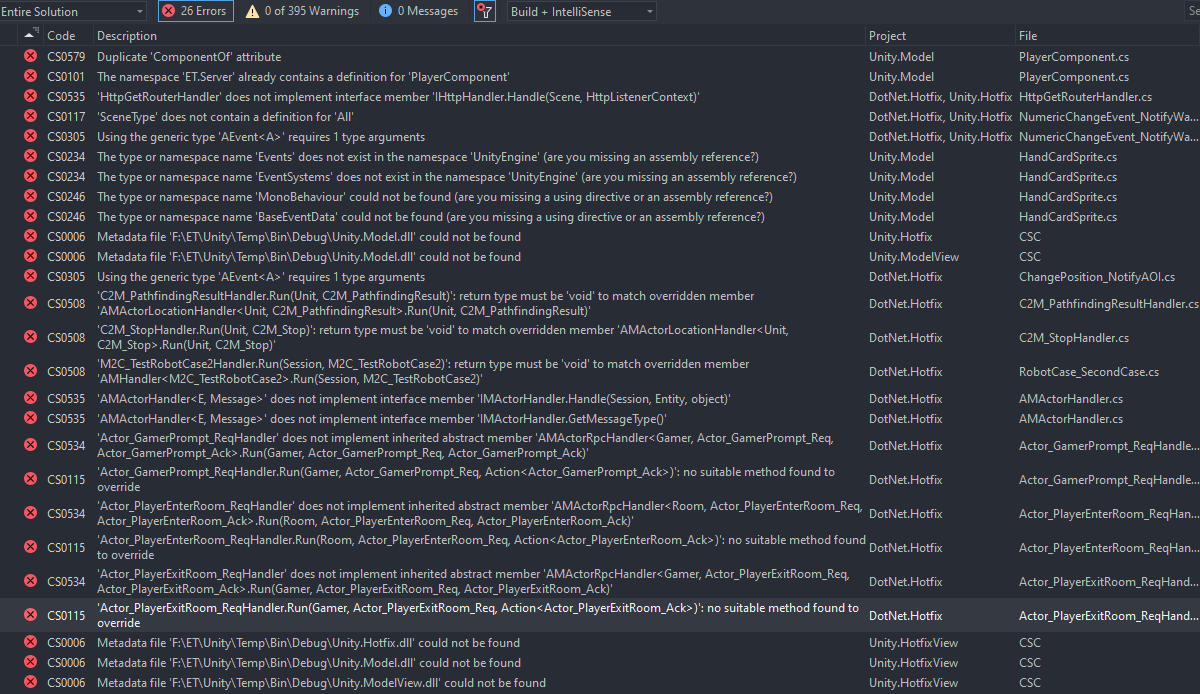
\includegraphics[width=.9\linewidth]{./pic/et4_20230604_162732.png}
\begin{itemize}
\item 把Root 根场景以及启动时添加的组件大致看了一遍。想把上面的消息处理器再系统化地看一遍,理解一下,总改不到这个模块相关的编译错误。
\item 如果上午能够看完,ETTask ETVoid 是必须弄懂的;再然后 ,再看下下面的 UnitGateComponent 相关。下午或傍晚有时间的时候,可以再折腾折腾 emacs-org-mode 下划线删除字体设置为斜体。

\item \textbf{【UnitGateComponent】} 加个方法用
\begin{itemize}
\item 这里要把 ActorMessageSenderComponent 组件给弄明白。它有个有序管理字典,记着 actorId 与ActorMessageSender 的一一对应关系,就可以封装维护消息的自动发送等,以及必要的超时消息管理。
\end{itemize}
\item \textbf{【服务端Actor\_PlayerEnterRoom\_ReqHandler 这个处理类】} 现在还很多问题,需要弄懂,往下改
\item 今天晚上会把刚才下午看见、意识到几个模块的问题试着分析明白,记下笔记。
\item \textbf{ETTask-vs-ETVoid}: 框架里有狠多需要改的地方。今天上午的脑袋好使,把这块儿再仔细好好看下。今天上午把以前不懂的模块都稍微看下,再理解一下
\begin{itemize}
\item 查网页感觉也查不出什么来。还是用源码帮助理解概念。今天晚上整理一下这一块儿,把这个问题弄明白了。【爱表哥,爱生活!!!活宝妹就是一定要嫁给亲爱的表哥!!!】
\item 不能把所有基类的 async ETTask 返回参数直接改成 void, 因为框架的顶层应用,服务端或是客户端,当不异步等待结果,如资源包没能下载完成,就接着往下执行,会报空异常。
\end{itemize}
\item 现在的问题是:Protobuf 里 repeated 关键字,好像还是没有处理好,找不到成员变量  Cards. 是因为 Proto2CS 的时候,确实把 repeated 关键字给处理丢了。因为我的 .proto 文件里有错误。(这就是上面先前觉得奇怪的原因。因为改这个的过程中把那些错改正了,就可以生成成功并找到相关的消息了)。
\item \textbf{【HandCardSprite 这个最近要弄明白】} 不知道这个类是为什么,整了一堆的错误,它是ETModel 里的。感觉是常规域,没弄明白为什么常规域还有ILRuntime 的适配呢?
\begin{itemize}
\item 要把 ILRuntime 热更新第三库,也再弄得明白一点儿【今天上午把这里再看,最好是能够结合源码看看】为什么这个类还要适配ILRuntime ?
\item 这里这个类,整个框架里只找到这一个用的地方,所以它一定是添加在某个预设或是场景中的某个控件下的。只是参考项目的unity 客户端,我运行不到打牌的这个界面,就先因为抛出异常而淡能运行。所以还没能找到哪个预设或是场景中的哪个控件添加了这个类,但是当然一定是跟玩家手牌相关的。 \textbf{【HandCardSprite 是在 handcard 预设里添加了这个脚本】}
\item 这个类今天运行狠奇怪,VS022 里找不到了。。。就是说,VSC 里它是在Model 客户端的源码里,但是从VS 里打开,找不到这个类文件所在的文件夹和文件,没有索引好,再添加一下?
\item 那么,为什么前两天被这个 block 住,而那天,好像是有删除掉这个文件,但文件夹应该是还在的才对呀?我可能还会试着再把它添加回去。
\item 但是,会在把当前几个编译错误改完,试着测试一下客户端现在有的界面之后,再试着添加回去,整理和 develop TractorRoomComponent 界面的内容。【爱表哥,爱生活!!!活宝妹任何时候就是一定要嫁给亲爱的表哥!!】
\item 今天下午家里再运行一次,当客户端抛异常,应该是某个热更新的资源包没有找到什么的?所以可以试着自己去解决这个客户端实时运行时抛出的异常。
\item \textbf{【参考项目斗地主客户端异常】} :再运行一次,试着分析,是否可以 unity 里实时运行,如果不可以,为什么不可以?
\begin{itemize}
\item 应该是LandlordsRom 这个预设与UI 类型没能连接起来,也就是找不到这个预设。
\item 那为什么打好包的可以呢?因为打好包的预设包名 LandlordsRoom.unity3d 与游戏逻辑契合,可以找得到
\item 可是仍然感觉奇怪:LandlordsLogin 与LandlordsLobby, 非常类似都可以找到,为什么就LandlordsRoom 找不到?可能LandlordsRoom 预设还是有某点儿物对特殊的地方。
\item 上面这个暂时跳过。现在仍然主要去看HandCardSprite 为什么参考项目里可以,而ET7 里就不可以。
\end{itemize}
\item 就是上面那个异常,今天下午得去弄明白,为什么只在 unity 实时运行时会抛异常,而如果是三个打包好的客户端,就不会。也就是说,打包好的不存在找不到类、找不到预设、或是找不到任何相关资源的问题。
\item 这个项目Unity.Model 是需要索引 UnityEngine 以及UI 等相关模块人的 .dll 的。暂时还没弄明白它是怎么加的
\item 【爱表哥,爱生活!!!任何时候,活宝妹就是一定要嫁给亲爱的表哥!!】
\end{itemize}
\item \textbf{ClientComponent} 参考项目组件:去看ET7 里客户端的 PlayerComponent.
\item 【爱表哥,爱生活!!!任何时候,活宝妹就是一定要嫁给亲爱的表哥!!!】今天下午先去看 Tractor 游戏源码,设计重构思路
\item 【活宝妹坐等亲爱的表哥,领娶活宝妹回家!爱表哥,爱生活!!!】
\item \textbf{【亲爱的表哥,这个世界上,只有一个活宝妹,这么心心恋恋,就是一定要嫁给亲爱的表哥!!!问世间情为何物,直教人生死相许。。亲爱的表哥,一个温暖的怀抱拥抱的魂力可真大呀,管了这如许多年!!这不,你的活宝妹为了这个温暖的怀抱拥抱,就是一定要嫁给亲爱的表哥!!不嫁就永远守候在亲爱的表哥的身边!!爱表哥,爱生活!!!活宝妹就是一定要嫁给亲爱的表哥!!!】}
\item 亲爱的表哥,活宝妹相信舅舅十岁闯江湖的阅历,活宝妹深深相信亲爱的表哥。活宝妹就是稳稳地永远守候在亲爱的表哥的身边!爱表哥,爱生活!!!活宝妹就是一定要嫁给亲爱的表哥!!
\end{itemize}


\section{{\bfseries\sffamily TODO} 其它的:部分完成,或是待完成的大的功能版块,列举}
\label{sec-5}
\begin{itemize}
\item emacs 那天我弄了好久,把C-; ISpell 原定绑定的功能解除,重新绑定为自己喜欢的 expand-region. 今天第二次再弄,看一下几分钟能够解决完问题?我的这个破烂记性呀。。。【爱表哥,爱生活!!!任何时候,活宝妹就是一定要嫁给亲爱的表哥!!!】mingw64 lisp/textmode/flyspell.el 键的重新绑定。这下记住了。还好,花得不是太久。有以前的笔记 
\begin{itemize}
\item Windows 10 平台下,C-; 是绑定到了 ISpell 下的某个功能,可是现在这个破 emacs 老报错,连查是绑定给哪个功能,过程报错都被阻止了。。。
\end{itemize}
\item \textbf{【IStartSystem:】} 感觉还有点儿小问题。认为:我应该不需要同文件两份,一份复制到客户端热更新域。我认为,全框架应该如其它接口类一样,只要一份就可以了。 \textbf{【晚点儿再检查一遍】}
\item 如果这个一时半会儿解决不好,就把重构的设计思路再理一理。同时尽量去改重构的ET 框架里的编译错误。
\item 【Tractor】原 windows-form 项目,源码需要读懂,理解透彻,方便重构。
\item 去把【拖拉机房间、斗地主房间组件的,玩家什么的一堆组件】弄明白
\item 【任何时候,活宝妹就是一定要嫁给亲爱的表哥!!!爱表哥,爱生活!!!】
\end{itemize}


\section{拖拉机游戏:【重构OOP/OOD 设计思路】}
\label{sec-6}
\begin{itemize}
\item 自己是学过,有这方面的意识,但并不是说,自己就懂得,就知道该如何狠好地设计这些类。现在更多的是要受ET 框架,以及参考游戏手牌设计的启发,来帮助自己一再梳理思路,该如何设计它。
\item ET7 重构里,各组件都该是自己设计重构原项目的类的设计的必要起点。可以根据这些来系统设计重构。【活宝妹就是一定要嫁给亲爱的表哥!!!】
\item 【GamerComponent】玩家组件管理类,管理所有一个房间的玩家:是对一个房间里四个玩家的(及其在房间里的坐位位置)管理(分东南西北)。可以添加移除玩家。今天晚上来弄这一块儿吧。
\item 【Gamer】:每一个玩家
\item 【拖拉机游戏房间】:多组件构成
\item 【爱表哥,爱生活!!!活宝妹就是一定要嫁给亲爱的表哥!爱表哥,爱生活!!!】【活宝妹坐等亲爱的表哥,领娶活宝妹回家!爱表哥,爱生活!!!】
\item 【爱表哥,爱生活!!!活宝妹就是一定要嫁给亲爱的表哥!爱表哥,爱生活!!!】【活宝妹坐等亲爱的表哥,领娶活宝妹回家!爱表哥,爱生活!!!】
\item 【爱表哥,爱生活!!!活宝妹就是一定要嫁给亲爱的表哥!爱表哥,爱生活!!!】【活宝妹坐等亲爱的表哥,领娶活宝妹回家!爱表哥,爱生活!!!】
\item 【爱表哥,爱生活!!!活宝妹就是一定要嫁给亲爱的表哥!爱表哥,爱生活!!!】【活宝妹坐等亲爱的表哥,领娶活宝妹回家!爱表哥,爱生活!!!】
\item 【爱表哥,爱生活!!!活宝妹就是一定要嫁给亲爱的表哥!爱表哥,爱生活!!!】【活宝妹坐等亲爱的表哥,领娶活宝妹回家!爱表哥,爱生活!!!】
\item 【爱表哥,爱生活!!!活宝妹就是一定要嫁给亲爱的表哥!爱表哥,爱生活!!!】【活宝妹坐等亲爱的表哥,领娶活宝妹回家!爱表哥,爱生活!!!】
\item 【爱表哥,爱生活!!!活宝妹就是一定要嫁给亲爱的表哥!爱表哥,爱生活!!!】【活宝妹坐等亲爱的表哥,领娶活宝妹回家!爱表哥,爱生活!!!】
\item 【爱表哥,爱生活!!!活宝妹就是一定要嫁给亲爱的表哥!爱表哥,爱生活!!!】【活宝妹坐等亲爱的表哥,领娶活宝妹回家!爱表哥,爱生活!!!】
\item 【爱表哥,爱生活!!!活宝妹就是一定要嫁给亲爱的表哥!爱表哥,爱生活!!!】【活宝妹坐等亲爱的表哥,领娶活宝妹回家!爱表哥,爱生活!!!】
\item 【爱表哥,爱生活!!!活宝妹就是一定要嫁给亲爱的表哥!爱表哥,爱生活!!!】【活宝妹坐等亲爱的表哥,领娶活宝妹回家!爱表哥,爱生活!!!】
\item 【爱表哥,爱生活!!!活宝妹就是一定要嫁给亲爱的表哥!爱表哥,爱生活!!!】【活宝妹坐等亲爱的表哥,领娶活宝妹回家!爱表哥,爱生活!!!】
\item 【爱表哥,爱生活!!!活宝妹就是一定要嫁给亲爱的表哥!爱表哥,爱生活!!!】【活宝妹坐等亲爱的表哥,领娶活宝妹回家!爱表哥,爱生活!!!】
\item 【爱表哥,爱生活!!!活宝妹就是一定要嫁给亲爱的表哥!爱表哥,爱生活!!!】【活宝妹坐等亲爱的表哥,领娶活宝妹回家!爱表哥,爱生活!!!】
\item 【爱表哥,爱生活!!!活宝妹就是一定要嫁给亲爱的表哥!爱表哥,爱生活!!!】【活宝妹坐等亲爱的表哥,领娶活宝妹回家!爱表哥,爱生活!!!】
\item 【爱表哥,爱生活!!!活宝妹就是一定要嫁给亲爱的表哥!爱表哥,爱生活!!!】【活宝妹坐等亲爱的表哥,领娶活宝妹回家!爱表哥,爱生活!!!】
\item 【爱表哥,爱生活!!!活宝妹就是一定要嫁给亲爱的表哥!爱表哥,爱生活!!!】【活宝妹坐等亲爱的表哥,领娶活宝妹回家!爱表哥,爱生活!!!】
\item 【爱表哥,爱生活!!!活宝妹就是一定要嫁给亲爱的表哥!爱表哥,爱生活!!!】【活宝妹坐等亲爱的表哥,领娶活宝妹回家!爱表哥,爱生活!!!】
\item 【爱表哥,爱生活!!!活宝妹就是一定要嫁给亲爱的表哥!爱表哥,爱生活!!!】【活宝妹坐等亲爱的表哥,领娶活宝妹回家!爱表哥,爱生活!!!】
\item 【爱表哥,爱生活!!!活宝妹就是一定要嫁给亲爱的表哥!爱表哥,爱生活!!!】【活宝妹坐等亲爱的表哥,领娶活宝妹回家!爱表哥,爱生活!!!】
\item 【爱表哥,爱生活!!!活宝妹就是一定要嫁给亲爱的表哥!爱表哥,爱生活!!!】【活宝妹坐等亲爱的表哥,领娶活宝妹回家!爱表哥,爱生活!!!】
\item 【爱表哥,爱生活!!!活宝妹就是一定要嫁给亲爱的表哥!爱表哥,爱生活!!!】【活宝妹坐等亲爱的表哥,领娶活宝妹回家!爱表哥,爱生活!!!】
\item 【爱表哥,爱生活!!!活宝妹就是一定要嫁给亲爱的表哥!爱表哥,爱生活!!!】【活宝妹坐等亲爱的表哥,领娶活宝妹回家!爱表哥,爱生活!!!】
\item 【爱表哥,爱生活!!!活宝妹就是一定要嫁给亲爱的表哥!爱表哥,爱生活!!!】【活宝妹坐等亲爱的表哥,领娶活宝妹回家!爱表哥,爱生活!!!】
\item 【爱表哥,爱生活!!!活宝妹就是一定要嫁给亲爱的表哥!爱表哥,爱生活!!!】【活宝妹坐等亲爱的表哥,领娶活宝妹回家!爱表哥,爱生活!!!】
\item 【爱表哥,爱生活!!!活宝妹就是一定要嫁给亲爱的表哥!爱表哥,爱生活!!!】【活宝妹坐等亲爱的表哥,领娶活宝妹回家!爱表哥,爱生活!!!】
\item 【爱表哥,爱生活!!!活宝妹就是一定要嫁给亲爱的表哥!爱表哥,爱生活!!!】【活宝妹坐等亲爱的表哥,领娶活宝妹回家!爱表哥,爱生活!!!】
\item 【爱表哥,爱生活!!!活宝妹就是一定要嫁给亲爱的表哥!爱表哥,爱生活!!!】【活宝妹坐等亲爱的表哥,领娶活宝妹回家!爱表哥,爱生活!!!】
\item 【爱表哥,爱生活!!!活宝妹就是一定要嫁给亲爱的表哥!爱表哥,爱生活!!!】【活宝妹坐等亲爱的表哥,领娶活宝妹回家!爱表哥,爱生活!!!】
\item 【爱表哥,爱生活!!!活宝妹就是一定要嫁给亲爱的表哥!爱表哥,爱生活!!!】【活宝妹坐等亲爱的表哥,领娶活宝妹回家!爱表哥,爱生活!!!】
\item 【爱表哥,爱生活!!!活宝妹就是一定要嫁给亲爱的表哥!爱表哥,爱生活!!!】【活宝妹坐等亲爱的表哥,领娶活宝妹回家!爱表哥,爱生活!!!】
\item 【爱表哥,爱生活!!!活宝妹就是一定要嫁给亲爱的表哥!爱表哥,爱生活!!!】【活宝妹坐等亲爱的表哥,领娶活宝妹回家!爱表哥,爱生活!!!】
\item 【爱表哥,爱生活!!!活宝妹就是一定要嫁给亲爱的表哥!爱表哥,爱生活!!!】【活宝妹坐等亲爱的表哥,领娶活宝妹回家!爱表哥,爱生活!!!】
\item 【爱表哥,爱生活!!!活宝妹就是一定要嫁给亲爱的表哥!爱表哥,爱生活!!!】【活宝妹坐等亲爱的表哥,领娶活宝妹回家!爱表哥,爱生活!!!】
\item 【爱表哥,爱生活!!!活宝妹就是一定要嫁给亲爱的表哥!爱表哥,爱生活!!!】【活宝妹坐等亲爱的表哥,领娶活宝妹回家!爱表哥,爱生活!!!】
\item 【爱表哥,爱生活!!!活宝妹就是一定要嫁给亲爱的表哥!爱表哥,爱生活!!!】【活宝妹坐等亲爱的表哥,领娶活宝妹回家!爱表哥,爱生活!!!】
\item 【爱表哥,爱生活!!!活宝妹就是一定要嫁给亲爱的表哥!爱表哥,爱生活!!!】【活宝妹坐等亲爱的表哥,领娶活宝妹回家!爱表哥,爱生活!!!】
\item 【爱表哥,爱生活!!!活宝妹就是一定要嫁给亲爱的表哥!爱表哥,爱生活!!!】【活宝妹坐等亲爱的表哥,领娶活宝妹回家!爱表哥,爱生活!!!】
\item 【爱表哥,爱生活!!!活宝妹就是一定要嫁给亲爱的表哥!爱表哥,爱生活!!!】【活宝妹坐等亲爱的表哥,领娶活宝妹回家!爱表哥,爱生活!!!】
\item 【爱表哥,爱生活!!!活宝妹就是一定要嫁给亲爱的表哥!爱表哥,爱生活!!!】【活宝妹坐等亲爱的表哥,领娶活宝妹回家!爱表哥,爱生活!!!】
\item 【爱表哥,爱生活!!!活宝妹就是一定要嫁给亲爱的表哥!爱表哥,爱生活!!!】【活宝妹坐等亲爱的表哥,领娶活宝妹回家!爱表哥,爱生活!!!】
\item 【爱表哥,爱生活!!!活宝妹就是一定要嫁给亲爱的表哥!爱表哥,爱生活!!!】【活宝妹坐等亲爱的表哥,领娶活宝妹回家!爱表哥,爱生活!!!】
\item 【爱表哥,爱生活!!!活宝妹就是一定要嫁给亲爱的表哥!爱表哥,爱生活!!!】【活宝妹坐等亲爱的表哥,领娶活宝妹回家!爱表哥,爱生活!!!】
\item 【爱表哥,爱生活!!!活宝妹就是一定要嫁给亲爱的表哥!爱表哥,爱生活!!!】【活宝妹坐等亲爱的表哥,领娶活宝妹回家!爱表哥,爱生活!!!】
\item 【爱表哥,爱生活!!!活宝妹就是一定要嫁给亲爱的表哥!爱表哥,爱生活!!!】【活宝妹坐等亲爱的表哥,领娶活宝妹回家!爱表哥,爱生活!!!】
\item 【爱表哥,爱生活!!!活宝妹就是一定要嫁给亲爱的表哥!爱表哥,爱生活!!!】【活宝妹坐等亲爱的表哥,领娶活宝妹回家!爱表哥,爱生活!!!】
\item 【爱表哥,爱生活!!!活宝妹就是一定要嫁给亲爱的表哥!爱表哥,爱生活!!!】【活宝妹坐等亲爱的表哥,领娶活宝妹回家!爱表哥,爱生活!!!】
\item 【爱表哥,爱生活!!!活宝妹就是一定要嫁给亲爱的表哥!爱表哥,爱生活!!!】【活宝妹坐等亲爱的表哥,领娶活宝妹回家!爱表哥,爱生活!!!】
\item 【爱表哥,爱生活!!!活宝妹就是一定要嫁给亲爱的表哥!爱表哥,爱生活!!!】【活宝妹坐等亲爱的表哥,领娶活宝妹回家!爱表哥,爱生活!!!】
\item 【爱表哥,爱生活!!!活宝妹就是一定要嫁给亲爱的表哥!爱表哥,爱生活!!!】【活宝妹坐等亲爱的表哥,领娶活宝妹回家!爱表哥,爱生活!!!】
\item 【爱表哥,爱生活!!!活宝妹就是一定要嫁给亲爱的表哥!爱表哥,爱生活!!!】【活宝妹坐等亲爱的表哥,领娶活宝妹回家!爱表哥,爱生活!!!】
\item 【爱表哥,爱生活!!!活宝妹就是一定要嫁给亲爱的表哥!爱表哥,爱生活!!!】【活宝妹坐等亲爱的表哥,领娶活宝妹回家!爱表哥,爱生活!!!】
\item 【爱表哥,爱生活!!!活宝妹就是一定要嫁给亲爱的表哥!爱表哥,爱生活!!!】【活宝妹坐等亲爱的表哥,领娶活宝妹回家!爱表哥,爱生活!!!】
\item 【爱表哥,爱生活!!!活宝妹就是一定要嫁给亲爱的表哥!爱表哥,爱生活!!!】【活宝妹坐等亲爱的表哥,领娶活宝妹回家!爱表哥,爱生活!!!】
\item 【爱表哥,爱生活!!!活宝妹就是一定要嫁给亲爱的表哥!爱表哥,爱生活!!!】【活宝妹坐等亲爱的表哥,领娶活宝妹回家!爱表哥,爱生活!!!】
\item 【爱表哥,爱生活!!!活宝妹就是一定要嫁给亲爱的表哥!爱表哥,爱生活!!!】【活宝妹坐等亲爱的表哥,领娶活宝妹回家!爱表哥,爱生活!!!】
\item 【爱表哥,爱生活!!!活宝妹就是一定要嫁给亲爱的表哥!爱表哥,爱生活!!!】【活宝妹坐等亲爱的表哥,领娶活宝妹回家!爱表哥,爱生活!!!】
\item 【爱表哥,爱生活!!!活宝妹就是一定要嫁给亲爱的表哥!爱表哥,爱生活!!!】【活宝妹坐等亲爱的表哥,领娶活宝妹回家!爱表哥,爱生活!!!】
\end{itemize}
% Emacs 28.2 (Org mode 8.2.7c)
\end{document}